\documentclass[10pt,fleqn]{article} % Default font size and left-justified equations
\usepackage[%
    pdftitle={Exercices de SII},
    pdfauthor={Xavier Pessoles}]{hyperref}
\usepackage{afterpage}
\usepackage{cancel}
\usepackage{subcaption}
\newcommand\blankpage{%
    \null
    \thispagestyle{empty}%
    \addtocounter{page}{-1}%
    \newpage}
    
\newcommand{\repRel}{../../../}
\input{\repRel/Style/packages}
\input{\repRel/Style/new_style}
\input{\repRel/Style/macros_SII}
\input{\repRel/Style/environment}


\usepackage{pdfpages}
\newcommand{\macrocomp}{macro_competences}
\newcommand{\comp}{competences}
\newcommand{\td}{fichier_td}
\newcommand{\repExo}{dossier}
\newcommand{\repStyle}{\repRel/Style}

\renewcommand{\repExo}{\repRel/Sujets_Concours/2017/XENS-PSI-2017-RobotVolc}
\graphicspath{{\repStyle/png/}{\repExo/images/}}

\def\discipline{Sciences \\Industrielles de \\ l'Ingénieur}
\def\xxtete{Sciences Industrielles de l'Ingénieur}

\def\numds{DS 3}
\def\classe{PSI$\star$}
\def\xxnumpartie{{\numds}}%\textsf{\textsf{Cy. 4, 6 \& 7}}}
\def\xxpartie{Devoir surveillé 3}

\def\xxnumchapitre{3 novembre 2025\vspace{.2cm} $\;$ }
\def\xxchapitre{\hspace{.12cm} }

%
\def\xxtitreexo{\noindent Plateau cyclique \& Robot Lola}
\def\xxsourceexo{\hspace{.2cm}  }


\def\xxposongletx{2}
\def\xxposonglettext{1.45}
\def\xxposonglety{20}
%\def\xxonglet{Part. 1 -- Ch. 3}
\def\xxonglet{\textsf{\numds}}%\textsf{\textsf{Cy. 4, 6 \& 7}}}
\def\xxactivite{\textsf{\numds}}
\def\xxauteur{\textsl{Xavier Pessoles}}

\def\xxcompetences{%
\textsl{%
%\textbf{Savoirs et compétences :}\\
}}

\renewcommand{\repExo}{../../../Sujets_Concours/2017/CCS-MP-2017-MesuresTopographiques}
\graphicspath{{\repStyle/png/}{\repExo/images/}{images/}}

\def\xxfigures{
\begin{center}
%\includegraphics[width=0.6\textwidth]{img_01}
\end{center}}%figues de la page de garde


\def\xxpied{%
\xxnumpartie -- \xxtitreexo\\
\xxactivite%
}

\setcounter{secnumdepth}{5}
%---------------------------------------------------------------------------

\usepackage{pgfplots}
\begin{document}
%\defimages{images}
%\chapterimage{png/Fond_Cin}
\input{\repRel/Style/new_pagegarde}
\vspace{5.5cm}
\pagestyle{fancy}
\thispagestyle{plain}

\def\columnseprulecolor{\color{ocre}}
\setlength{\columnseprule}{0.4pt} 



\def\xxactivite{}
\def\xxnumactivite{}
\def\xxdate{3 novembre 2025}


\normaltrue
\newpage
\proffalse \colletrue
%\proftrue

\input{\repStyle/pagegarde_SII_DS.tex}

\vspace{5cm}

\proftrue
%\proffalse


\graphicspath{{\repStyle/png/}{../../../Sujets_Concours/2005/EA_Plateau/images/}{../../../Sujets_Concours/2015/CCMP_PSI_Lola/images/}}


\section*{Questions de TP}

Soit un déplacement commandé par un trapèze de vitesse. La distance parcourue est notée $L$, l'accélération maximale est notée $\indice{a}{max}$ et la vitesse maximale est notée $\indice{v}{max}$.

\question{Tracer les allures de la postion, de la vitesse et de l'accélération en fonction du temps.}
\ifprof
\begin{center}
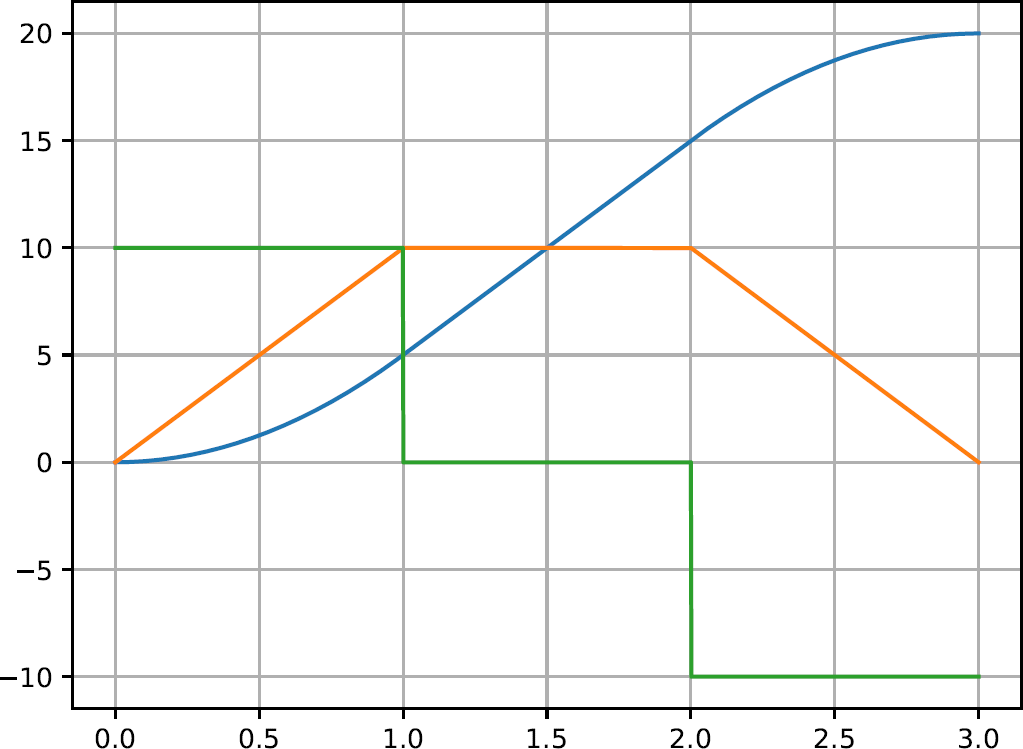
\includegraphics[width=.5\linewidth]{Q_01.png}
\end{center}
\else
\fi

On souhaite réaliser une distance $L$ en un temps $T$. On fait l'hypothèse que l'accélération maximale est toujours atteinte. Le temps pour accélérer et décélérer sont identiques. Enfin, on se place dans le cas, où le palier de vitesse ($\indice{v}{max}$ ou $\indice{v}{F}$) sera atteint.

\question{Exprimer les temps $t_1$ et $t_2$ (respectivement fins de la phase 1 et de la phase 2) ainsi que la vitesse atteinte $V_F$ en fin de première phase.}
\ifprof
\begin{corrige}
On  a :
\begin{itemize}
\item $T=t_2 + t_1$
\item $t_2 V_F = L$
\item $\indice{a}{max} =\dfrac{V_F}{t_1}$.
\end{itemize}
On a donc $T-\dfrac{L}{V_F} - \dfrac{V_F}{\indice{a}{max}} = 0$
$ \Rightarrow TV_F-L - \dfrac{V_F^2}{\indice{a}{max}} = 0$
$ \Rightarrow  V_F^2 -TV_F\indice{a}{max}+L\indice{a}{max} = 0$
$ \Rightarrow  \Delta = T^2\indice{a}{max}^2 - 4L\indice{a}{max} $

On a alors $V_F = \dfrac{T\indice{a}{max}\pm \sqrt{T^2\indice{a}{max}^2 - 4L\indice{a}{max}}}{2}$
\end{corrige}
\else
\fi

Soit une liste de temps \lstinline{les_t} et une liste de vitesses \lstinline{les_v}. 

\question{Donner, en Python, les instructions pemettant de calculer la liste de positions \lstinline{les_x} en utilisant la méthode des trapèzes. Vous vous appuierez sur un schéma.}
\ifprof
\begin{minipage}[c]{.55\linewidth}
\begin{lstlisting}
def calcule_les_x(les_t:[float], les_v:[float])->[float] :
    les_x = [0]
    x = 0
    for i in range(len(les_t)-1):
        x = x+.5*(les_v[i+1]+les_v[i])*(les_t[i+1]-les_t[i])
        les_x.append(x)
    return les_x
\end{lstlisting}
\end{minipage}\hfill
\begin{minipage}[c]{.4\linewidth}
\begin{center}
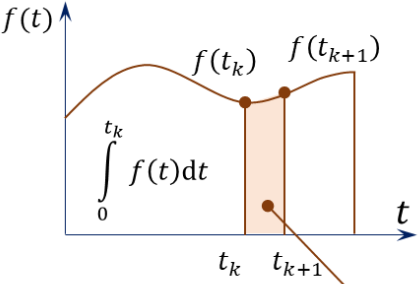
\includegraphics[width=.95\linewidth]{Q_03.png}
\end{center}
\end{minipage}

\else
\fi

\input{../../../Sujets_Concours/2005/EA_Plateau/2005_EA_Plateau.tex}

\input{../../../Sujets_Concours/2015/CCMP_PSI_Lola/CCMP_PSI_Lola_P2_DS.tex}


\end{document}



